
\section{Exercises}

%\Comment{need to add in conceptual questions about ci for mean, such as 9-12 of original 04e.tex from openintro }

%__________________
\subsection{Inference for a single mean with the $t$-distribution}

% 1

\eoce{\qt{Identify the critical $t$}\ \videohref{ahss_eoce_sol-identify_critical_t}\ \ A random sample is selected from an approximately normal population with unknown standard deviation. Find the degrees of freedom and the critical $t$-value (t$^\star$) for the given sample size and confidence level.\vspace{-3mm}
\begin{multicols}{2}
\begin{parts}
\item $n = 6$, CL = 90\%
\item $n = 21$, CL = 98\%
\item $n = 29$, CL = 95\%
\item $n = 12$, CL = 99\%
\end{parts}
\end{multicols}
}{}

% 2
 
\noindent \begin{minipage}[c]{0.5\textwidth}
\eoce{\qt{$t$-distribution} The figure on the right shows three unimodal and symmetric curves: the standard normal (z) distribution,  the $t$-distribution with 5 degrees of freedom, and the $t$-distribution with 1 degree of freedom. Determine which is which, and explain your reasoning.}
{}
\end{minipage}
\begin{minipage}[c]{0.48\textwidth}
\begin{center}
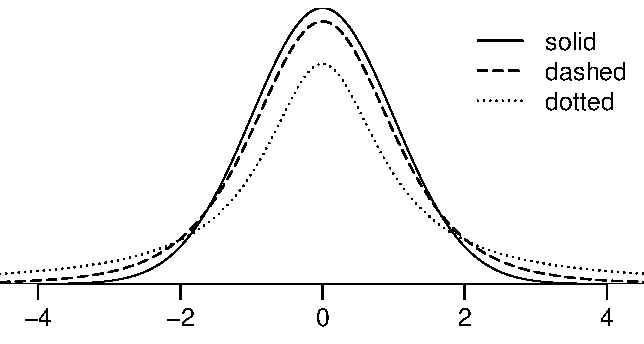
\includegraphics[width=0.93\textwidth]{ch_inference_for_means/figures/eoce/t_vs_z/t_vs_z}
\end{center}
\end{minipage}

% 3

\eoce{\qt{Find the p-value, Part I} An independent random sample is selected from an approximately normal population with an unknown standard deviation. Find the p-value for the given set of hypotheses and $T$ test statistic. Also determine if the null hypothesis would be rejected at $\alpha = 0.05$.\vspace{-3mm}
\begin{multicols}{2}
\begin{parts}
\item $H_A: \mu > \mu_0 $, $n = 11$, $T = 1.91$
\item $H_A: \mu < \mu_0 $, $n = 17$, $T = -3.45$
\item $H_A: \mu \ne \mu_0 $, $n = 7$, $T = 0.83$
\item $H_A: \mu > \mu_0 $, $n = 28$, $T = 2.13$
\end{parts}
\end{multicols}
}{}

% 4

\eoce{\qt{Find the p-value, Part II} An independent random sample is selected from an approximately normal population with an unknown standard deviation. Find the p-value for the given set of hypotheses and $T$ test statistic. Also determine if the null hypothesis would be rejected at $\alpha = 0.01$.
\begin{parts}
\item $H_A: \mu > 0.5$, $n = 26$, $T = 2.485$
\item $H_A: \mu < 3$, $n = 18$, $T = 0.5$
\end{parts}
}{}


% 5

\eoce{\qt{Working backwards, Part I} A 95\% confidence interval for a population mean, $\mu$, is given as (18.985, 21.015). This confidence interval is based on a simple random sample of 36 observations. Calculate the sample mean and standard deviation. Assume that all conditions necessary for inference are satisfied. Use the $t$-distribution in any calculations.
}{}

% 6

\eoce{\qt{Working backwards, Part II} A 90\% confidence interval for a population mean is (65, 77). The population distribution is approximately normal and the population standard deviation is unknown. This confidence interval is based on a simple random sample of 25 observations. Calculate the sample mean, the margin of error, and the sample standard deviation.
}{}

\textA{\newpage}

% 7

\eoce{\qt{Sleep habits of New Yorkers} \label{NewYorkSleep} New York is known as ``the city that never sleeps". A random sample of 25 New Yorkers were asked how much sleep they get per night. Statistical summaries of these data are shown below. Do these data provide strong evidence that New Yorkers sleep less than 8 hours a night on average?
\begin{center}
\begin{tabular}{rrrrrr}
 \hline
n 	& $\bar{x}$	& s		& min 	& max \\ 
 \hline
25 	& 7.73 		& 0.77 	& 6.17 	& 9.78 \\ 
  \hline
\end{tabular}
\end{center}

\begin{parts}
\item Write the hypotheses in symbols and in words.
\item Check conditions, then calculate the test statistic, $T$, and the associated degrees of freedom.
\item Find and interpret the p-value in this context. Drawing a picture may be helpful.
\item What is the conclusion of the hypothesis test?
\item If you were to construct a 90\% confidence interval that corresponded to this hypothesis test, would you expect 8 hours to be in the interval?
\end{parts}
}{}

% 8

\eoce{\qt{Fuel efficiency of Prius} Fueleconomy.gov, the official US government source for fuel economy information, allows users to share gas mileage information on their vehicles. The histogram below shows the distribution of gas mileage in miles per gallon (MPG) from 14 users who drive a 2012 Toyota Prius. The sample mean is 53.3 MPG and the standard deviation is 5.2 MPG. Note that these data are user estimates and since the source data cannot be verified, the accuracy of these estimates are not guaranteed.\footfullcite{data:prius}
\begin{center}
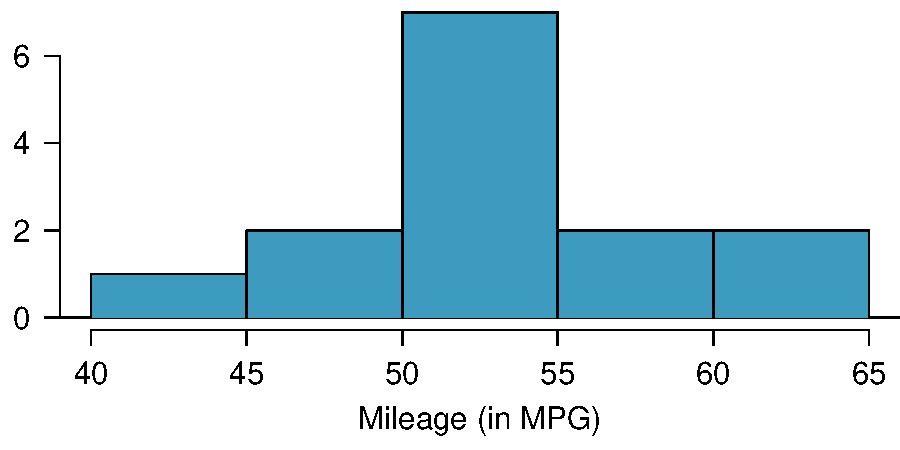
\includegraphics[width=0.6\textwidth]{ch_inference_for_means/figures/eoce/prius/prius_hist}
\end{center}
\begin{parts}
\item We would like to use these data to evaluate the average gas mileage of all 2012 Prius drivers. Do you think this is reasonable? Why or why not?
\item The EPA claims that a 2012 Prius gets 50 MPG (city and highway mileage combined). Do these data provide strong evidence against this estimate for drivers who participate on fueleconomy.gov? Note any assumptions you must make as you proceed with the test.
\item Calculate a 95\% confidence interval for the average gas mileage of a 2012 Prius by drivers who participate on fueleconomy.gov.
\end{parts}
}{}

% 9

\eoce{\qt{Find the mean} You are given the following hypotheses:
\begin{align*}
H_0&: \mu = 60 \\
H_A&: \mu < 60
\end{align*}
We know that the sample standard deviation is 8 and the sample size is 20. For what sample mean would the p-value be equal to 0.05? Assume that all conditions necessary for inference are satisfied.
}{}

% 10

\eoce{\qt{$t^\star$ vs. $z^\star$} For a given confidence level, $t^{\star}_{df}$ is larger than $z^{\star}$. Explain how $t^{*}_{df}$ being slightly larger than $z^{*}$ affects the width of the confidence interval.
}{}

% 11

\eoce{\qt{Play the piano}\ \videohref{ahss_eoce_sol-play_piano}\ \ Georgianna claims that in a small city renowned for its music school, the average child takes at least 5 years of piano lessons. We have a random sample of 20 children from the city, with a mean of 4.6 years of piano lessons and a standard deviation of 2.2 years.
\begin{parts}
\item Evaluate Georgianna's claim using a hypothesis test.
\item Construct a 95\% confidence interval for the number of years students in this city take piano lessons, and interpret it in context of the data.
\item Do your results from the hypothesis test and the confidence interval agree? Explain your reasoning.
\end{parts}
}{}

% 12

\eoce{\qt{Auto exhaust and lead exposure} Researchers interested in lead exposure due to car exhaust sampled the blood of 52 police officers subjected to constant inhalation of automobile exhaust fumes while working traffic enforcement in a primarily urban environment. The blood samples of these officers had an average lead concentration of 124.32 $\mu$g/l  and a SD of 37.74 $\mu$g/l; a previous study of individuals from a nearby suburb, with no history of exposure, found an average blood level concentration of 35 $\mu$g/l.\footfullcite{Mortada:2000}
\begin{parts}
\item Write down the hypotheses that would be appropriate for testing if the police officers appear to have been exposed to a higher concentration of lead.
\item Explicitly state and check all conditions necessary for inference on these data.
\item Test the hypothesis that the downtown police officers have a higher lead exposure than the group in the previous study. Interpret your results in context.
\item Based on your preceding result, without performing a calculation, would a 99\% confidence interval for the average blood concentration level of police officers contain 35 $\mu$g/l?
\end{parts}
}{}

% 13

\eoce{\qt{Car insurance savings}\  \videohref{ahss_eoce_sol-car_insurance_savings}\ \ A market researcher wants to evaluate car insurance savings at a competing company. Based on past studies he is assuming that the standard deviation of savings is \$100. He wants to collect data such that he can get a margin of error of no more than \$10 at a 95\% confidence level. How large of a sample should he collect?
}{}

% 14

\eoce{\qt{SAT scores} SAT scores of students at an Ivy League college are distributed with a standard deviation of 250 points. Two statistics students, Raina and Luke, want to estimate the average SAT score of students at this college as part of a class project. They want their margin of error to be no more than 25 points.
\begin{parts}
\item Raina wants to use a 90\% confidence interval. How large a sample should she collect?
\item Luke wants to use a 99\% confidence interval. Without calculating the actual sample size, determine whether his sample should be larger or smaller than Raina's, and explain your reasoning.
\item Calculate the minimum required sample size for Luke.
\end{parts}
}{}

%__________________
\subsection{Inference for paired data}

%15

\eoce{\qt{Air quality} Air quality measurements were collected in a random sample of 25 country capitals in 2013, and then again in the same cities in 2014. We would like to use these data to compare average air quality between the two years.
\begin{parts}
\item Should we use a one-sided or a two-sided test? Explain your reasoning.
\item Should we use a paired or non-paired test? Explain your reasoning.
\item Should we use a $t$-test or a z-test? Explain your reasoning.
\end{parts}
}{}

\textA{\pagebreak}

% 16

\eoce{\qt{True / False: paired} Determine if the following statements about paired data are true or false. If false, explain.
\begin{parts}
\item In a paired analysis we first take the difference of each pair of observations, and then we do inference on these differences.
\item Two data sets of different sizes cannot be analyzed as paired data.
\item Each observation in one data set has a natural correspondence with exactly one observation from the other data set.
\item Each observation in one data set is subtracted from the average of the other data set's observations.
\end{parts}
}{}

% 17

\eoce{\qtq{Paired or not? Part I} In each of the following scenarios, determine if the data are paired.
\begin{parts}
\item Compare pre- (beginning of semester) and post-test (end of semester) scores of students.
\item Assess gender-related salary gap by comparing salaries of randomly sampled men and women.
\item Compare artery thicknesses at the beginning of a study and after 2 years of taking Vitamin E for the same group of patients.
\item Assess effectiveness of a diet regimen by comparing the before and after weights of subjects.
\end{parts}
}{}

% 18

\eoce{\qtq{Paired or not? Part II} In each of the following scenarios, determine if the data are paired.
\begin{parts}
\item We would like to know if Intel's stock and Southwest Airlines' stock have similar rates of return. To find out, we take a random sample of 50 days, and record Intel's and Southwest's stock on those same days.
\item We randomly sample 50 items from Target stores and note the price for each. Then we visit Walmart and collect the price for each of those same 50 items.
\item A school board would like to determine whether there is a difference in average SAT scores for students at one high school versus another high school in the district. To check, they take a simple random sample of 100 students from each high school.
\end{parts}
}{}

% 19

\eoce{\qt{Global warming, Part I} \label{warming} Is there strong evidence of global warming? Let's consider a small scale example, comparing how temperatures have changed in the US from 1968 to 2008. The daily high temperature reading on January 1 was collected in 1968 and 2008 for 51 randomly selected locations in the continental US. Then the difference between the two readings (temperature in 2008 - temperature in 1968) was calculated for each of the 51 different locations. The average of these 51 values was 1.1 degrees with a standard deviation of 4.9 degrees. We are interested in determining whether these data provide strong evidence of temperature warming in the continental US. 
\begin{parts}
\item Is there a relationship between the observations collected in 1968 and 2008? Or are the observations in the two groups independent? Explain.
\item Write hypotheses for this research in symbols and in words.
\item Check the conditions required to complete this test.
\item Calculate the test statistic and find the p-value.
\item What do you conclude? Interpret your conclusion in context.
\item What type of error might we have made? Explain in context what the error means.
\item Based on the results of this hypothesis test, would you expect a confidence interval for the average difference between the temperature measurements from 1968 and 2008 to include 0? Explain your reasoning.
\end{parts}
}{}

\textA{\pagebreak}

% 20

\eoce{\qt{High School and Beyond, Part I} \label{hsb2} The National Center of Education Statistics conducted a survey of high school seniors, collecting test data on reading, writing, and several other subjects. Here we examine a simple random sample of 200 students from this survey. Side-by-side box plots of reading and writing scores as well as a histogram of the differences in scores are shown below.
\begin{center}
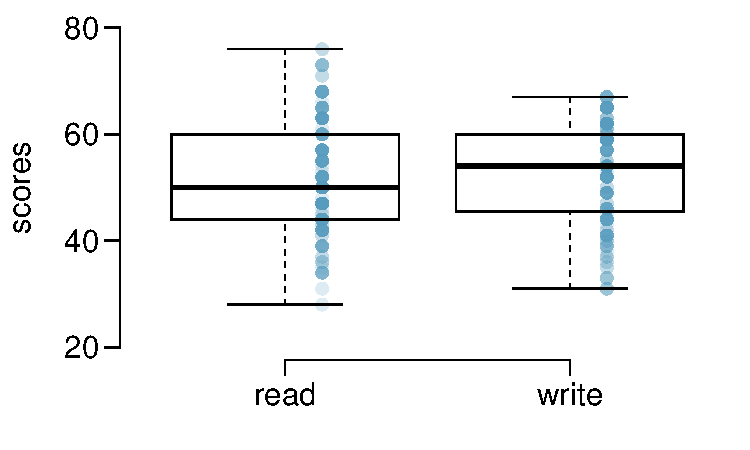
\includegraphics[width=0.44\textwidth]{ch_inference_for_means/figures/eoce/hsb2/hsb2_read_write_box}
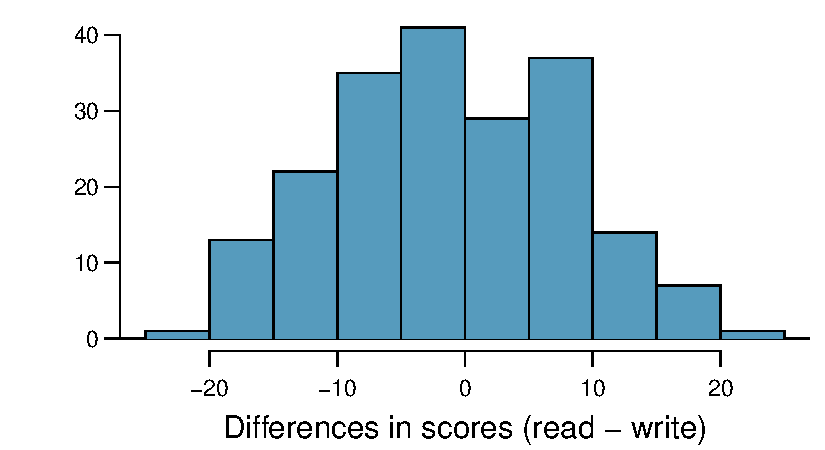
\includegraphics[width=0.54\textwidth]{ch_inference_for_means/figures/eoce/hsb2/hsb2_diff_hist}
\end{center}
\begin{parts}

\item Is there a clear difference in the average reading and writing scores?

\item Are the reading and writing scores of each student independent of each other?

\item Create hypotheses appropriate for the following research question: is there an evident difference in the average scores of students in the reading and writing exam?

\item Check the conditions required to complete this test.

\item The average observed difference in scores is $\bar{x}_{read-write} = -0.545$, and the standard deviation of the differences is 8.887 points. Do these data provide convincing evidence of a difference between the average scores on the two exams?
\item What type of error might we have made? Explain what the error means in the context of the application.
\item Based on the results of this hypothesis test, would you expect a confidence interval for the average difference between the reading and writing scores to include 0? Explain your reasoning.
\end{parts}
}{}

% 21

\eoce{\qt{Global warming, Part II} We considered the differences between the temperature readings in January 1 of 1968 and 2008 at 51 locations in the continental US in Exercise~\ref{warming}. The mean and standard deviation of the reported differences are 1.1 degrees and 4.9 degrees.
\begin{parts}
\item Calculate a 90\% confidence interval for the average difference between the temperature measurements between 1968 and 2008.
\item Interpret this interval in context.
\item Does the confidence interval provide convincing evidence that the temperature was higher in 2008 than in 1968 in the continental US? Explain.
\end{parts}
}{}

 % 22

\eoce{\qt{High school and beyond, Part II} We considered the differences between the reading and writing scores of a random sample of 200 students who took the High School and Beyond Survey in Exercise~\ref{hsb2}. The mean and standard deviation of the differences are $\bar{x}_{read-write} = -0.545$ and 8.887 points.
\begin{parts}
\item Calculate a 95\% confidence interval for the average difference between the reading and writing scores of all students.
\item Interpret this interval in context.
\item Does the confidence interval provide convincing evidence that there is a real difference in the average scores? Explain.
\end{parts}
}{}

\textA{\pagebreak}

% 23

\eoce{\qt{Gifted children} Researchers collected a simple random sample of 36 children who had been identified as gifted in a large city. The following histograms show the distributions of the IQ scores of mothers and fathers of these children. Also provided are some sample statistics.\footfullcite{Graybill:1994}

\begin{center}
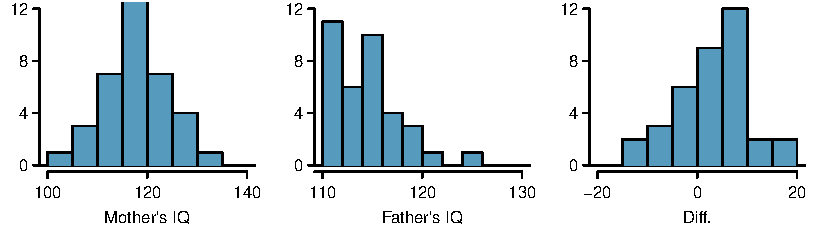
\includegraphics[width=0.9\textwidth]{ch_inference_for_means/figures/eoce/gifted/gifted_IQ_hist} \\[2mm]
{\small
\begin{tabular}{r | c c c}
		& Mother	& Father	& Diff. \\
\hline
Mean	& 118.2 	& 114.8	& 3.4 \\
SD		& 6.5		& 3.5		& 7.5 \\
n		& 36		& 36		& 36
\end{tabular}
}
\end{center}

\begin{parts}
\item Are the IQs of mothers and the IQs of fathers in this data set related? Explain.
\item Conduct a hypothesis test to evaluate if the scores are equal on average. Make sure to clearly state your hypotheses, check the relevant conditions, and state your conclusion in the context of the data.
\end{parts}
}{}

% 24

\eoce{\qt{Sample size and pairing} Determine if the following statement is true or false, and if false, explain your reasoning: If comparing means of two groups with equal sample sizes, always use a paired test.}
{}


\textA{\newpage}

%__________________
\subsection{Difference of two means using the $t$-distribution}

% 25

\eoce{\qt{Cleveland vs. Sacramento} Average income varies from one region of the country to another, and it often reflects both lifestyles and regional living expenses. Suppose a new graduate is considering a job in two locations, Cleveland, OH and Sacramento, CA, and he wants to see whether the average income in one of these cities is higher than the other. He would like to conduct a hypothesis test based on two small samples from the 2000 Census, but he first must consider whether the conditions are met to implement the test. Below are histograms for each city. Should he move forward with the hypothesis test? Explain your reasoning. \\
\begin{minipage}[c]{0.7\textwidth}
\begin{center}
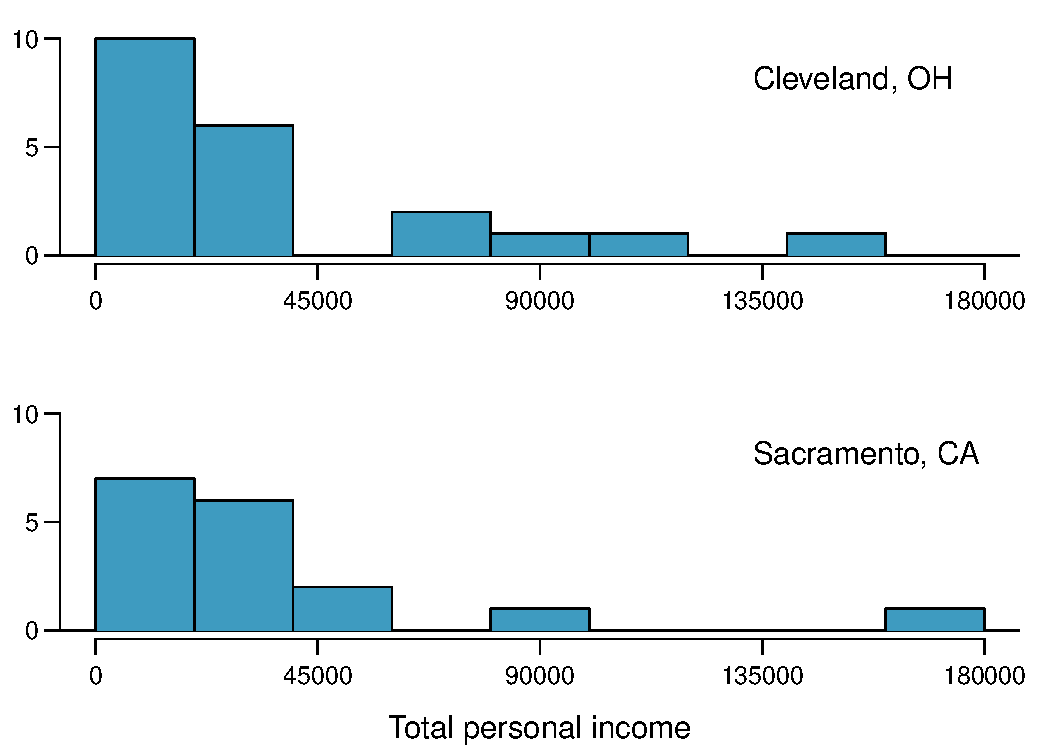
\includegraphics[width=0.95\textwidth]{ch_inference_for_means/figures/eoce/cleSac/cleSac_hist}
\end{center}
\end{minipage}
\begin{minipage}[c]{0.3\textwidth}
{\small
\begin{tabular}{l c}
\hline
		& Cleveland, OH	\\
\hline
Mean 	& \$ 35,749		\\
SD 		& \$ 39,421		\\
n 		& 21				
\end{tabular}

\vspace{2cm}

\begin{tabular}{l c}
\hline
		& Sacramento, CA \\
\hline
Mean	& \$ 35,500 \\
SD		& \$ 41,512 \\
n		& 17
\end{tabular}
}
\end{minipage}
}{}

% 26

\eoce{\qt{Oscar winners} The first Oscar awards for best actor and best actress were given out in 1929. The histograms below show the age distribution for all of the best actor and best actress winners from 1929 to 2012. Summary statistics for these distributions are also provided. Is a hypothesis test appropriate for evaluating whether the difference in the average ages of best actors and actresses might be due to chance? Explain your reasoning. \footfullcite{data:oscars} \\
\begin{minipage}[c]{0.72\textwidth}
\begin{center}
 \href{\oiRedirectUrl{tableau_oscar_winners}}{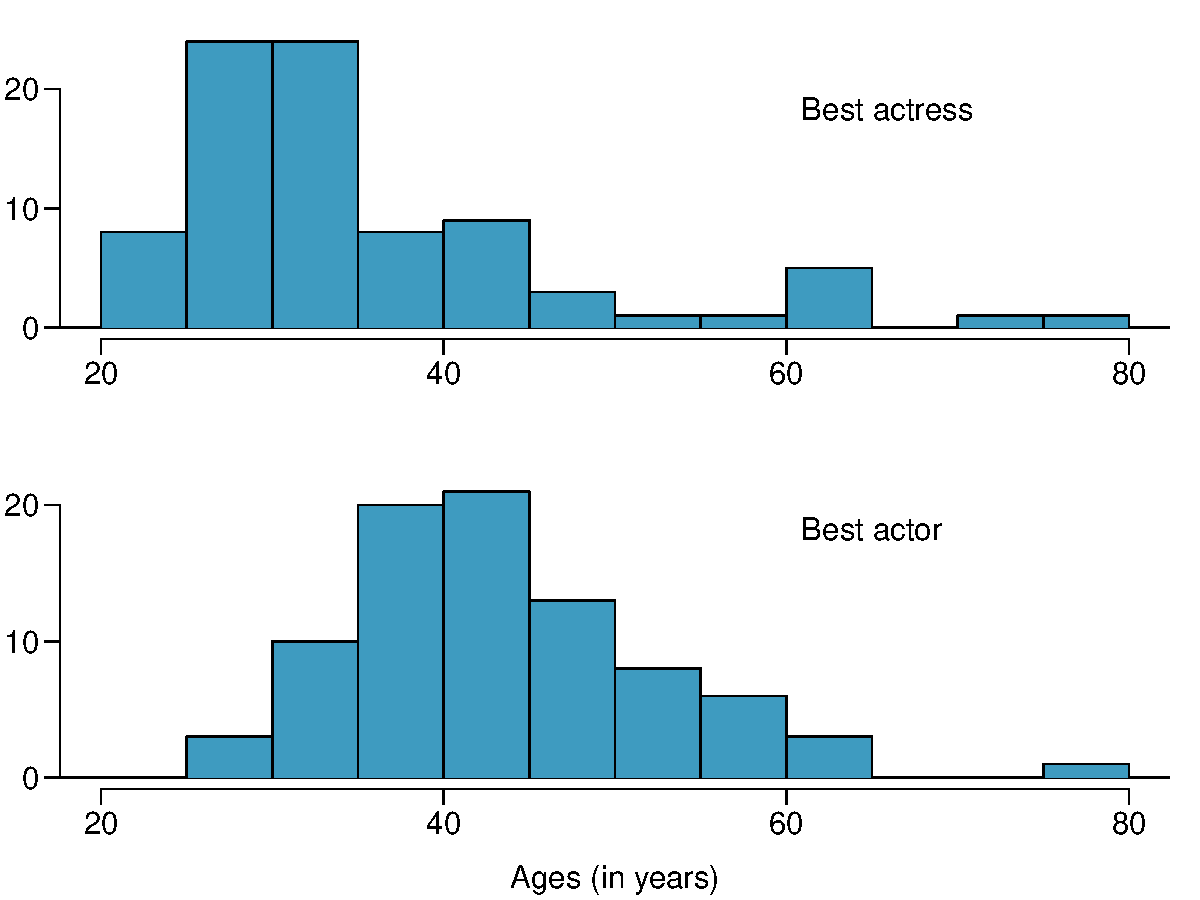
\includegraphics[width=0.95\textwidth]{ch_inference_for_means/figures/eoce/oscars/oscars_Hist}}
\end{center}
\end{minipage}
\begin{minipage}[c]{0.27\textwidth}
{\small
\begin{tabular}{l c}
\hline
		& Best Actress	\\
\hline
Mean 	& 35.6		\\
SD 		& 11.3		\\
n 		& 84			\\	
		& \\
		& \\
		& \\
		& \\
		& \\
\hline
		& Best Actor \\
\hline
Mean	& 44.7 \\
SD		& 8.9 \\
n		& 84
\end{tabular}
}
\end{minipage}
}{}

% 27

\eoce{\qt{Friday the 13$^{\text{th}}$, Part I} \label{fridayTraffic} In the early 1990's, researchers in the UK collected data on traffic flow, number of shoppers, and traffic accident related emergency room admissions on Friday the 13$^{\text{th}}$ and the previous Friday, Friday the 6$^{\text{th}}$. The normal probability plots below show the distribution of number of cars passing by a specific intersection on Friday the 6$^{\text{th}}$ and Friday the 13$^{\text{th}}$ for many such date pairs. Also given are some sample statistics, where the difference is the number of cars on the 6th minus the number of cars on the 13th.\footfullcite{Scanlon:1993}
\begin{center}
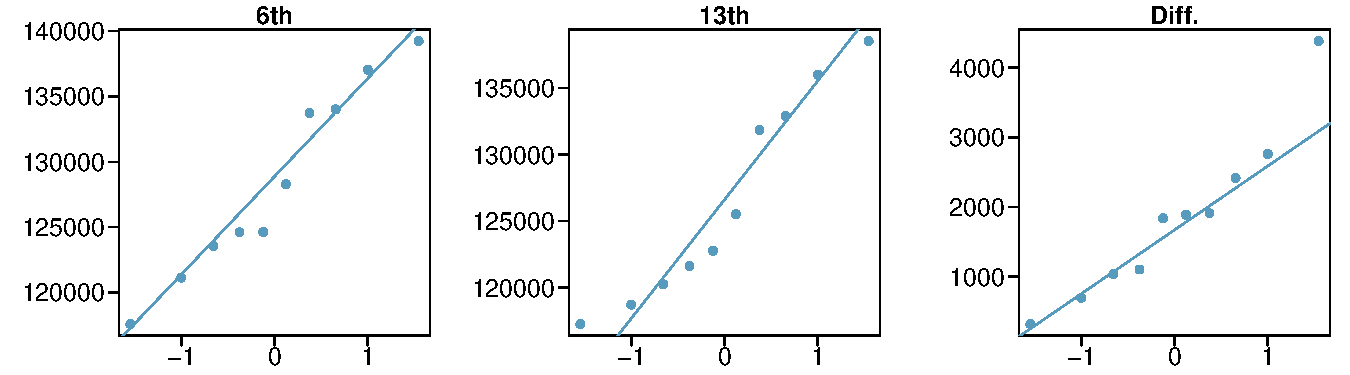
\includegraphics[width=0.9\textwidth]{ch_inference_for_means/figures/eoce/friday/friday_traffic_qq} \\
$\:$ \\
{\small
\begin{tabular}{l c c c}
\hline
		& 6$^{\text{th}}$	& 13$^{\text{th}}$ 	& Diff.\\
\hline	
$\bar{x}$ 	&128,385			& 126,550 		& 1,835 \\
$s$		&7,259			& 7,664			& 1,176 \\
$n$		&10				& 10				& 10 \\
\hline
\end{tabular}
}
\end{center}
\begin{parts}
\item Are there any underlying structures in these data that should be considered in an analysis? Explain.
\item What are the hypotheses for evaluating whether the number of people out on Friday the 6$^{\text{th}}$ is different than the number out on Friday the 13$^{\text{th}}$?
\item Check conditions to carry out the hypothesis test from part~(b).
\item Calculate the test statistic and the p-value.
\item What is the conclusion of the hypothesis test?
\item Interpret the p-value in this context.
\item What type of error might have been made in the conclusion of your test? Explain.
\end{parts}
}{}

% 28

\eoce{\qt{Diamonds, Part I} \label{diamonds} Prices of diamonds are determined by what is known as the 4 Cs: cut, clarity, color, and carat weight. The prices of diamonds go up as the carat weight increases, but the increase is not smooth. For example, the difference between the size of a 0.99 carat diamond and a 1 carat diamond is undetectable to the naked human eye, but the price of a 1 carat diamond tends to be much higher than the price of a 0.99 diamond. In this question we use two random samples of diamonds, 0.99 carats and 1 carat, each sample of size 23, and compare the average prices of the diamonds. In order to be able to compare equivalent units, we first divide the price for each diamond by 100 times its weight in carats. That is, for a 0.99 carat diamond, we divide the price by 99. For a 1 carat diamond, we divide the price by 100. The distributions and some sample statistics are shown below.\footfullcite{ggplot2} \\[1mm]
\begin{minipage}[c]{0.6\textwidth}
Conduct a hypothesis test to evaluate if there is a difference between the average standardized prices of 0.99 and 1 carat diamonds. Make sure to state your hypotheses clearly, check relevant conditions, and interpret your results in context of the data. \\[2mm]
\begin{tabular}{l c c }
\hline
		& 0.99 carats	 	& 1 carat\\
\hline	
Mean 	& \$ 44.51			& \$ 56.81			 \\
SD		& \$ 13.32			&\$ 16.13			 \\
n		&23				& 23 \\
\hline
\end{tabular}
\end{minipage}%
\begin{minipage}[c]{0.4\textwidth}
\begin{center}
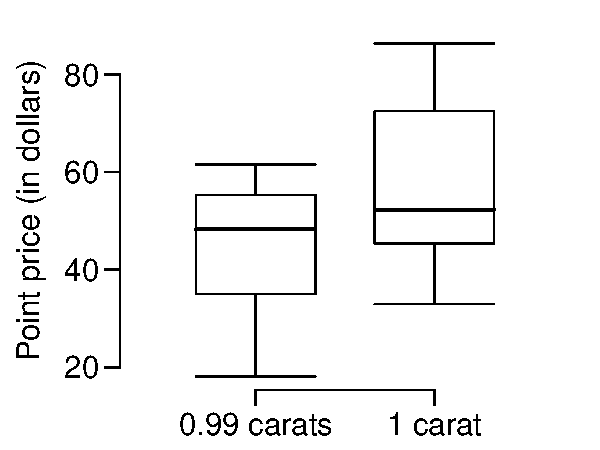
\includegraphics[width=0.85\textwidth]{ch_inference_for_means/figures/eoce/diamonds/diamonds_box}
\end{center}
\end{minipage}
}{}

% 29

\eoce{\qt{Friday the 13$^{\text{th}}$, Part II}\label{fridayAccident}\  \videohref{ahss_eoce_sol-friday_13th_accident}\ \ The Friday the $13^{th}$ study reported in Exercise~\ref{fridayTraffic} also provides data on traffic accident related emergency room admissions. The distributions of these counts from Friday the 6$^{\text{th}}$ and Friday the 13$^{\text{th}}$ are shown below for six such paired dates along with summary statistics. You may assume that conditions for inference are met.

\begin{center}
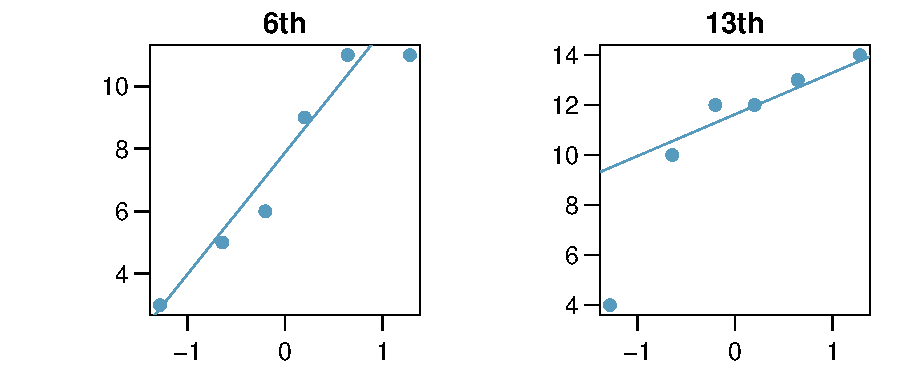
\includegraphics[width=0.74\textwidth]{ch_inference_for_means/figures/eoce/friday/friday_acc_qq} \\
$\:$ \\
\begin{minipage}[c]{0.36\textwidth}
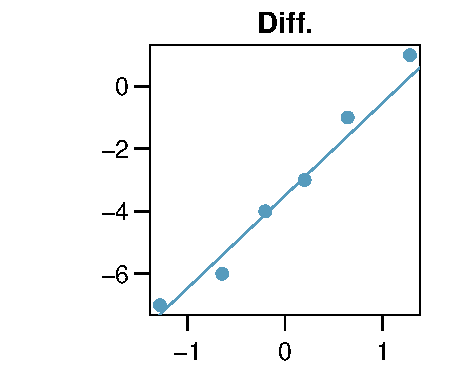
\includegraphics[width=\textwidth]{ch_inference_for_means/figures/eoce/friday/friday_acc_qq1}
\end{minipage}
\begin{minipage}[c]{0.36\textwidth}
\ \ \begin{tabular}{l c c c}
\hline
		& 6$^{\text{th}}$	& 13$^{\text{th}}$ 	& diff\\
\hline	
Mean 	&7.5				& 10.83 			& -3.33 \\
SD		&3.33			& 3.6				& 3.01 \\
n		&6				& 6				& 6 \\
\hline
\end{tabular}
\end{minipage}
\end{center}

\begin{parts}
\item Conduct a hypothesis test to evaluate if there is a difference between the average numbers of traffic accident related emergency room admissions between Friday the 6$^{\text{th}}$ and Friday the~13$^{\text{th}}$.
\item Calculate a 95\% confidence interval for the difference between the average numbers of traffic accident related emergency room admissions between Friday the 6$^{\text{th}}$ and Friday the 13$^{\text{th}}$.
\item The conclusion of the original study states, ``Friday 13th is unlucky for some. The risk of hospital admission as a result of a transport accident may be increased by as much as 52\%. Staying at home is recommended.'' Do you agree with this statement? Explain your reasoning.
\end{parts}
}{}

% 30

\eoce{\qt{Diamonds, Part II} In Exercise~\ref{diamonds}, we discussed diamond prices (standardized by weight) for diamonds with weights 0.99 carats and 1 carat. See the table for summary statistics, and then construct a 95\% confidence interval for the average difference between the standardized prices of 0.99 and 1 carat diamonds. You may assume the conditions for inference are met.
\begin{center}
\begin{tabular}{l c c }
\hline
		& 0.99 carats	 	& 1 carat\\
\hline	
Mean 	& \$ 44.51			& \$ 56.81			 \\
SD		& \$ 13.32			&\$ 16.13			 \\
n		&23				& 23 \\
\hline
\end{tabular}
\end{center}
}{}

\textA{\newpage}

% 31

\eoce{\qt{Chicken diet and weight, Part I}\label{chicks}\ \videohref{ahss_eoce_sol-chick_wts_linseed_horsebean}\ \ Chicken farming is a multi-billion dollar industry, and any methods that increase the growth rate of young chicks can reduce consumer costs while increasing company profits, possibly by millions of dollars. An experiment was conducted to measure and compare the effectiveness of various feed supplements on the growth rate of chickens. Newly hatched chicks were randomly allocated into six groups, and each group was given a different feed supplement. Below are some summary statistics from this data set along with box plots showing the distribution of weights by feed type. \footfullcite{data:chickwts}

\noindent\begin{minipage}[c]{0.65\textwidth}
\begin{center}
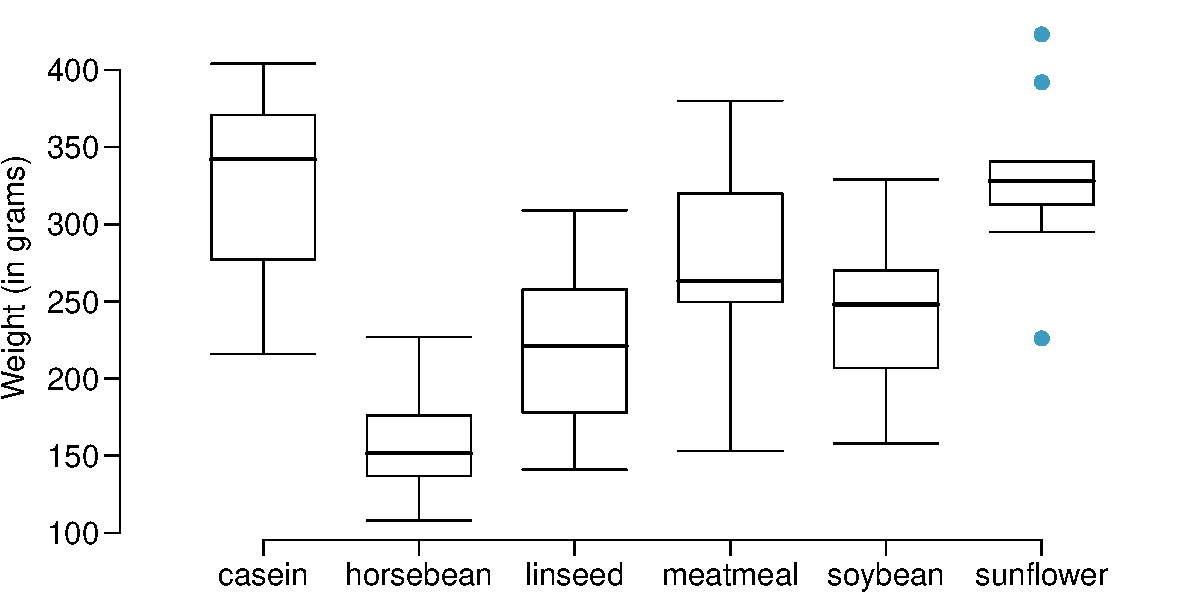
\includegraphics[width= \textwidth]{ch_inference_for_means/figures/eoce/chicks/chicks_box}
\end{center}
\end{minipage}
\begin{minipage}[c]{0.35\textwidth}
{\footnotesize\begin{tabular}{l c c c}
\hline
       		& Mean		& SD		& n \\
\hline
casein  		& 323.58 		& 64.43	& 12 \\
horsebean 	& 160.20 		& 38.63	& 10 \\
linseed  		& 218.75 		& 52.24	& 12 \\
meatmeal 	& 276.91 		& 64.90	& 11 \\
soybean  		& 246.43 		& 54.13	& 14 \\
sunflower 		& 328.92 		& 48.84	& 12 \\
\hline
\end{tabular}}
\end{minipage} 

\begin{parts}
\item Describe the distributions of weights of chickens that were fed linseed and horsebean.
\item Do these data provide strong evidence that the average weights of chickens that were fed linseed and horsebean are different? Use a 5\% significance level.
\item What type of error might we have committed? Explain.
\item Would your conclusion change if we used $\alpha = 0.01$?
\end{parts}
}{}

% 32

\eoce{\qt{Fuel efficiency of manual and automatic cars, Part I} \label{fuelEff} Each year the US Environmental Protection Agency (EPA) releases fuel economy data on cars manufactured in that year. Below are summary statistics on fuel efficiency (in miles/gallon) from random samples of cars with manual and automatic transmissions manufactured in 2012. Do these data provide strong evidence of a difference between the average fuel efficiency of cars with manual and automatic transmissions in terms of their average city mileage? Assume that conditions for inference are satisfied. \footfullcite{data:epaMPG}

\noindent\begin{minipage}[c]{0.38\textwidth}
\begin{center}
\begin{tabular}{l c c }
\hline
		& \multicolumn{2}{c}{City MPG} \\
\hline
       		& Automatic 	& Manual		 \\
Mean  	& 16.12    		& 19.85  	 \\
SD 		& 3.58    		& 4.51  	 \\
n		& 26			& 26 \\
\hline
& \\
& \\
\end{tabular}
\end{center}
\end{minipage}
\begin{minipage}[c]{0.6\textwidth}
\begin{center}
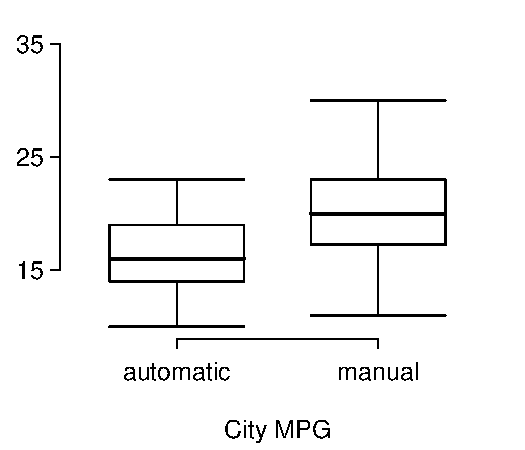
\includegraphics[width=0.7\textwidth]{ch_inference_for_means/figures/eoce/fuelEff/fuelEff_hist_city}
\end{center}
\end{minipage}
}{}

% 33

\eoce{\qt{Chicken diet and weight, Part II} \label{chicksCasein} Casein is a common weight gain supplement for humans. Does it have an effect on chickens? Using data provided in Exercise~\ref{chicks}, test the hypothesis that the average weight of chickens that were fed casein is different than the average weight of chickens that were fed soybean. If your hypothesis test yields a statistically significant result, discuss whether or not the higher average weight of chickens can be attributed to the casein diet. Assume that conditions for inference are satisfied.
}{}

% 34

\eoce{\qt{Fuel efficiency of manual and automatic cars, Part II} The table provides summary statistics on highway fuel economy of cars manufactured in 2012 (from Exercise~\ref{fuelEff}). Use these statistics to calculate a 98\% confidence interval for the difference between average highway mileage of manual and automatic cars, and interpret this interval in the context of the data.\footfullcite{data:epaMPG}

\noindent\begin{minipage}[c]{0.38\textwidth}
\begin{center}
\begin{tabular}{l c c }
\hline
		& \multicolumn{2}{c}{Hwy MPG} \\
\hline
       		& Automatic 	& Manual		 \\
Mean  	& 22.92   		& 27.88    		 \\
SD 		& 5.29     		& 5.01    		 \\
n		& 26			& 26 \\
\hline
& \\
& \\
\end{tabular}
\end{center}
\end{minipage}
\begin{minipage}[c]{0.6\textwidth}
\begin{center}
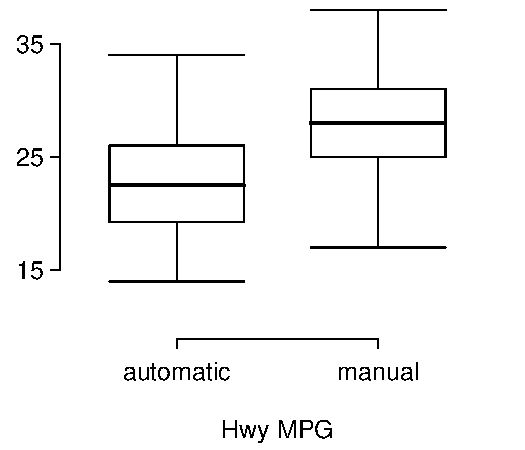
\includegraphics[width=0.7\textwidth]{ch_inference_for_means/figures/eoce/fuelEff/fuelEff_hist_hwy}
\end{center}
\end{minipage}
}{}

% 35

\eoce{\qt{Gaming and distracted eating, Part I} \label{gaming} A group of researchers are interested in the possible effects of distracting stimuli during eating, such as an increase or decrease in the amount of food consumption. To test this hypothesis, they monitored food intake for a group of 44 patients who were randomized into two equal groups. The treatment group ate lunch while playing solitaire, and the control group ate lunch without any added distractions. Patients in the treatment group ate 52.1 grams of biscuits, with a standard deviation of 45.1 grams, and patients in the control group ate 27.1 grams of biscuits, with a standard deviation of 26.4 grams. Do these data provide convincing evidence that the average food intake (measured in amount of biscuits consumed) is different for the patients in the treatment group? Assume that conditions for inference are satisfied. \footfullcite{Oldham:2011}
}{}

% 36

\eoce{\qt{Gaming and distracted eating, Part II} The researchers from Exercise~\ref{gaming} also investigated the effects of being distracted by a game on how much people eat. The 22 patients in the treatment group who ate their lunch while playing solitaire were asked to do a serial-order recall of the food lunch items they ate. The average number of items recalled by the patients in this group was 4.9, with a standard deviation of 1.8. The average number of items recalled by the patients in the control group (no distraction) was 6.1, with a standard deviation of 1.8. Do these data provide strong evidence that the average number of food items recalled by the patients in the treatment and control groups are different?
}{}

\textA{\newpage}

% 37

\eoce{\qt{Prison isolation experiment, Part I} \label{prison} Subjects from Central Prison in Raleigh,  NC, volunteered for an experiment involving an ``isolation'' experience. The goal of the experiment was to find a treatment that reduces subjects' psychopathic deviant $T$-scores. This score measures a person's need for control or their rebellion against control, and it is part of a commonly used mental health test called the Minnesota Multiphasic Personality Inventory (MMPI) test. The experiment had three treatment groups: 
\begin{enumerate}[(1)]
\setlength{\itemsep}{0mm}
\item Four hours of sensory restriction plus a 15 minute ``therapeutic"  tape advising that professional help is available.
\item Four hours of sensory restriction plus a 15 minute ``emotionally neutral'' tape on training hunting dogs.
\item Four hours of  sensory restriction but no taped message. 
\end{enumerate}
Forty-two subjects were randomly assigned to these treatment groups, and an MMPI test was administered before and after the treatment. Distributions of the differences between pre and post treatment scores (pre - post) are shown below, along with some sample statistics. Use this information to independently test the effectiveness of each treatment. Make sure to clearly state your hypotheses, check conditions, and interpret results in the context of the data.\footfullcite{data:prison}

\begin{center}
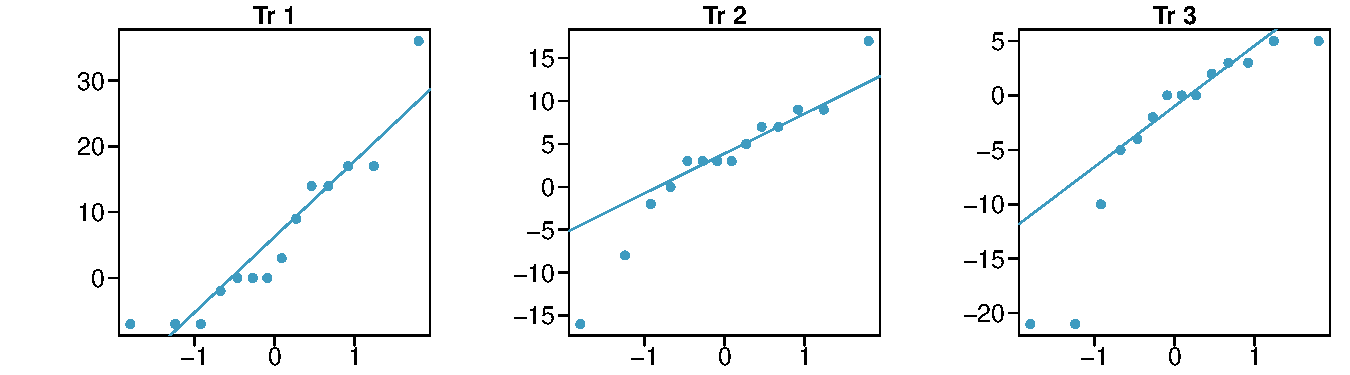
\includegraphics[width=\textwidth]{ch_inference_for_means/figures/eoce/prison/prison_qq} \\
$\:$ \\
\begin{tabular}{l  r  r  r  r  }
\hline
				& Tr 1	& Tr 2	& Tr 3		\\
\hline
Mean			& 6.21	& 2.86	& -3.21			  \\
SD				& 12.3	& 7.94	& 8.57		 \\
n				& 14		& 14		& 14 	 \\
\hline
\end{tabular}
\end{center}
}{}

% 38

\eoce{\qt{True / False: comparing means} Determine if the following statements are true or false, and explain your reasoning for statements you identify as false.
\begin{parts}
\item When comparing means of two samples where $n_1 = 20$ and $n_2 = 40$, we can use the normal model for the difference in means since $n_2 \ge 30$.
\item As the degrees of freedom increases, the $t$-distribution approaches normality.
\item We use a pooled standard error for calculating the standard error of the difference between means when sample sizes of groups are equal to each other.
\end{parts}
}{}


\textA{\newpage}

%__________________
\subsection{Comparing many means with ANOVA (special topic)}

% 39

\eoce{\qt{Fill in the blank} When doing an ANOVA, you observe large differences in means between groups. Within the ANOVA framework, this would most likely be interpreted as evidence strongly favoring the $\rule{2cm}{0.5pt}$ hypothesis.
}{}

% 40

\eoce{\qtq{Which test} We would like to test if students who are in the social sciences, natural sciences, arts and humanities, and other fields spend the same amount of time studying for this course. What type of test should we use? Explain your reasoning.
}{}

% 41

\eoce{\qt{Chicken diet and weight, Part III} In Exercises~\ref{chicks} and \ref{chicksCasein} we compared the effects of two types of feed at a time. A better analysis would first consider all feed types at once: casein, horsebean, linseed, meat meal, soybean, and sunflower. The ANOVA output below can be used to test for differences between the average weights of chicks on different diets.
\begin{center}
\begin{tabular}{lrrrrr}
\hline
 		& Df 	& Sum Sq		& Mean Sq 	& F value 	& Pr($>$F) \\ 
\hline
feed 		& 5 	& 231,129.16 	& 46,225.83 	& 15.36 	& 0.0000 \\ 
Residuals	& 65 & 195,556.02 	& 3,008.55	&  		&  \\ 
\hline
%\multicolumn{6}{r}{$s_{pooled} = 55.85$ on $df=65$}
\end{tabular}
\end{center}
Conduct a hypothesis test to determine if these data provide convincing evidence that the average weight of chicks varies across some (or all) groups. Make sure to check relevant conditions. Figures and summary statistics are shown below.

\begin{minipage}[c]{0.65\textwidth}
\begin{center}
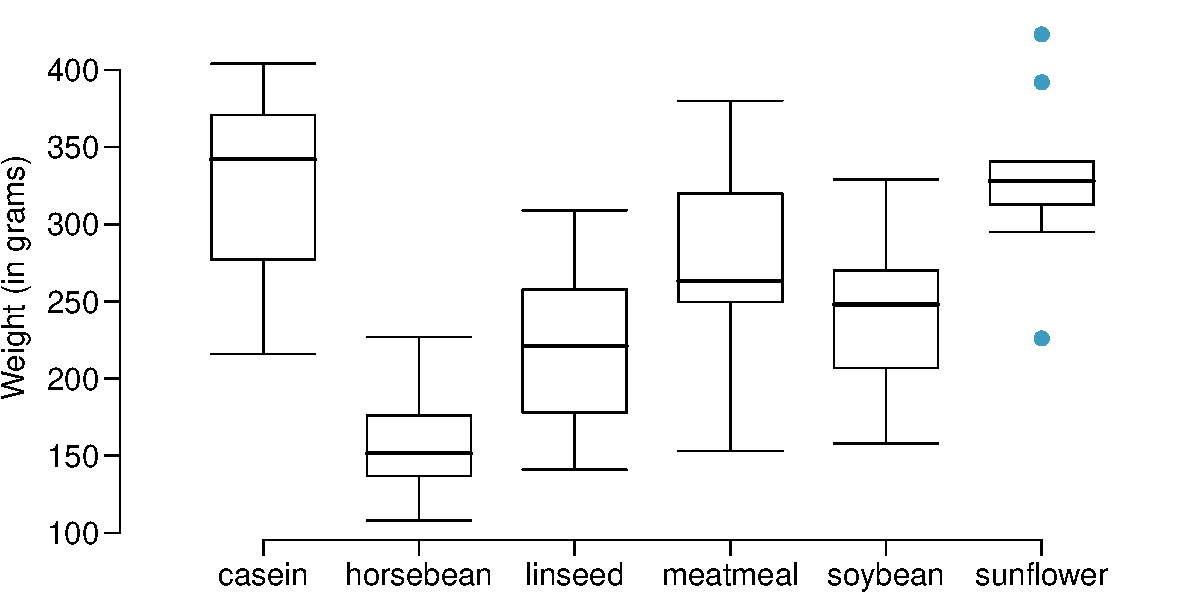
\includegraphics[width= \textwidth]{ch_inference_for_means/figures/eoce/chicks/chicks_box}
\end{center}
\end{minipage}
\begin{minipage}[c]{0.35\textwidth}
{\footnotesize\begin{tabular}{l c c c}
\hline
       		& Mean		& SD		& n \\
\hline
casein  		& 323.58 		& 64.43	& 12 \\
horsebean 	& 160.20 		& 38.63	& 10 \\
linseed  		& 218.75 		& 52.24	& 12 \\
meatmeal 	& 276.91 		& 64.90	& 11 \\
soybean  		& 246.43 		& 54.13	& 14 \\
sunflower 		& 328.92 		& 48.84	& 12 \\
\hline
\end{tabular}}
\end{minipage} 
}{}

% 42

\eoce{\qt{Teaching descriptive statistics} A study compared five different methods for teaching descriptive statistics. The five methods were traditional lecture and discussion, programmed textbook instruction, programmed text with lectures, computer instruction, and computer instruction with lectures. 45 students were randomly assigned, 9 to each method. After completing the course, students took a 1-hour exam. 
\begin{parts}
\item What are the hypotheses for evaluating if the average test scores are different for the different teaching methods?
\item What are the degrees of freedom associated with the $F$-test for evaluating these hypotheses?
\item Suppose the p-value for this test is 0.0168. What is the conclusion?
\end{parts}
}{}

\textA{\newpage}

% 43

\eoce{\qt{Coffee, depression, and physical activity} \label{coffeeDepression} Caffeine is the world's most widely used stimulant, with approximately 80\% consumed in the form of coffee. Participants in a study investigating the relationship between coffee consumption and exercise were asked to report the number of hours they spent per week on moderate (e.g., brisk walking) and vigorous (e.g., strenuous sports and jogging) exercise. Based on these data the researchers estimated the total hours of metabolic equivalent tasks (MET) per week, a value always greater than 0. The table below gives summary statistics of MET for women in this study based on the amount of coffee consumed.\footfullcite{Lucas:2011}
 
\begin{adjustwidth}{-4em}{-4em}

\begin{center}
\begin{tabular}{l  r  r  r  r  r  r}
\multicolumn{1}{c}{}	& \multicolumn{5}{c}{\textit{Caffeinated coffee consumption}} \\
\cline{2-6}
				& $\le$ 1 cup/week	& 2-6 cups/week	& 1 cup/day	& 2-3 cups/day & $\ge$ 4 cups/day & Total	\\
\hline
Mean			& 18.7	& 19.6	& 19.3	& 18.9	& 17.5 			  \\
SD				& 21.1	& 25.5	& 22.5	& 22.0	& 22.0 \\
n				& 12,215	& 6,617 		& 17,234	& 12,290	& 2,383 	& 50,739 \\
\hline
\end{tabular}
\end{center}
\end{adjustwidth}

\begin{parts}

\item Write the hypotheses for evaluating if the average physical activity level varies among the different levels of coffee consumption.

\item Check conditions and describe any assumptions you must make to proceed with the test.

\item Below is part of the output associated with this test. Fill in the empty cells.

\begin{center}
\renewcommand{\arraystretch}{1.25}
\begin{tabular}{lrrrrr}
  \hline
 			& Df 	& Sum Sq		& Mean Sq	& F value	& Pr($>$F) \\ 
  \hline
coffee	 	& \fbox{\textcolor{white}{{\footnotesize XXXXX}}}	 & \fbox{\textcolor{white}{{\footnotesize XXXXX}}} 		& \fbox{\textcolor{white}{{\footnotesize XXXXX}}} 			& \fbox{\textcolor{white}{{\footnotesize XXXXX}}} 	& 0.0003 \\ 
Residuals		& \fbox{\textcolor{white}{{\footnotesize XXXXX}}} & 25,564,819 	& \fbox{\textcolor{white}{{\footnotesize  XXXXX}}} 			&  		&  \\ 
   \hline
Total			& \fbox{\textcolor{white}{{\footnotesize XXXXX}}} &25,575,327
\end{tabular}
\end{center}

\item What is the conclusion of the test?

\end{parts}
}{}

% 44

\eoce{\qt{Student performance across discussion sections} A professor who teaches a large introductory statistics class (197 students) with eight discussion sections would like to test if student performance differs by discussion section, where each discussion section has a different teaching assistant. The summary table below shows the average final exam score for each discussion section as well as the standard deviation of scores and the number of students in each section.
\begin{center}
\begin{tabular}{rrrrrrrrr}
  \hline
 			& Sec 1 & Sec 2 & Sec 3 & Sec 4 & Sec 5 & Sec 6 & Sec 7 & Sec 8 \\ 
  \hline
$n_i$		& 33 & 19 & 10 & 29 & 33 & 10 & 32 & 31 \\ 
$\bar{x}_i$	& 92.94 & 91.11 & 91.80 & 92.45 & 89.30 & 88.30 & 90.12 & 93.35 \\ 
$s_i$ 		& 4.21 & 5.58 & 3.43 & 5.92 & 9.32 & 7.27 & 6.93 & 4.57 \\ 
   \hline
\end{tabular}
\end{center}
The ANOVA output below can be used to test for differences between the average scores from the different discussion sections.
\begin{center}
\begin{tabular}{lrrrrr}
\hline
 			& Df 		& Sum Sq & Mean Sq 	& F value & Pr($>$F) \\ 
\hline
section 		& 7 		& 525.01 	& 75.00 		& 1.87 	& 0.0767 \\ 
Residuals 	& 189	& 7584.11	& 40.13 		&  		&  \\ 
\hline
\end{tabular}
\end{center}
Conduct a hypothesis test to determine if these data provide convincing evidence that the average score varies across some (or all) groups. Check conditions and describe any assumptions you must make to proceed with the test.
}{}

\textA{\newpage}

% 45

\eoce{\qt{GPA and major} Undergraduate students taking an introductory statistics course at Duke University conducted a survey about GPA and major. The side-by-side box plots show the distribution of GPA among three groups of majors. Also provided is the ANOVA output.
\begin{center}
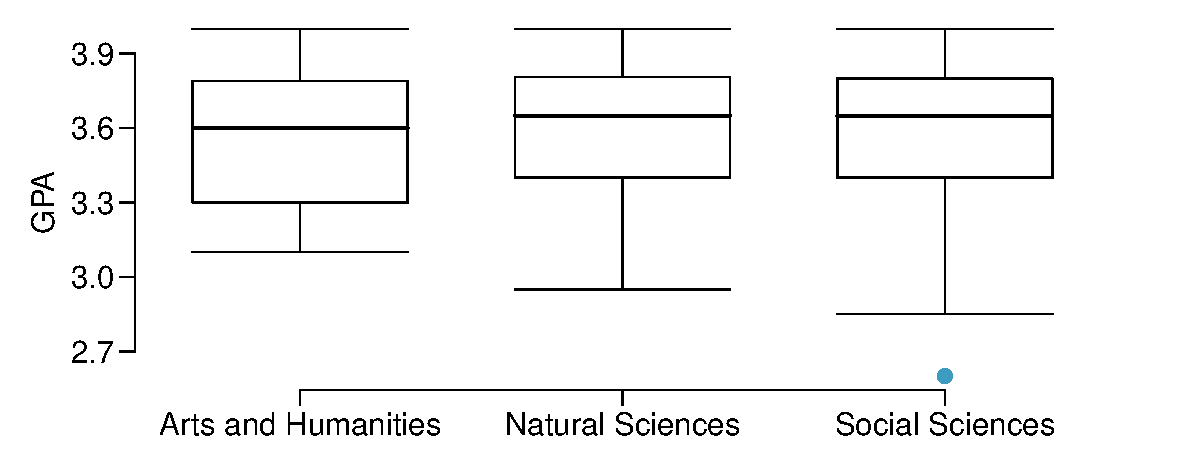
\includegraphics[width=0.85\textwidth]{ch_inference_for_means/figures/eoce/gpaMajor/gpaMajor_box}
\end{center}
\begin{center}
\begin{tabular}{lrrrrr}
  \hline
 & Df & Sum Sq & Mean Sq & F value & Pr($>$F) \\ 
  \hline
major & 2 & 0.03 & 0.02 & 0.21 & 0.8068 \\ 
  Residuals & 195 & 15.77 & 0.08 &  &  \\ 
   \hline
\end{tabular}
\end{center}
\begin{parts}
\item Write the hypotheses for testing for a difference between average GPA across majors.
\item What is the conclusion of the hypothesis test?
\item How many students answered these questions on the survey, i.e. what is the sample size?
\end{parts}
}{}

\textA{\newpage}

% 46

\eoce{\qt{Work hours and education} The General Social Survey collects data on demographics, education, and work, among many other characteristics of US residents. \footfullcite{data:gss:2010} Using ANOVA, we can consider educational attainment levels for all 1,172 respondents at once. Below are the distributions of hours worked by educational attainment and relevant summary statistics that will be helpful in carrying out this analysis.
\begin{center}

\begin{tabular}{l  r  r  r  r  r  r}
\multicolumn{1}{c}{}	& \multicolumn{5}{c}{\textit{Educational attainment}} \\
\cline{2-6}
				& Less than HS 	& HS		& Jr Coll	& Bachelor's & Graduate & Total	\\
\hline
Mean			& 38.67			& 39.6	& 41.39	& 42.55	& 40.85 	& 40.45			  \\
SD				& 15.81			& 14.97	& 18.1	& 13.62	& 15.51	& 15.17		 \\
n				& 121			& 546 	& 97		& 253	& 155 	& 1,172 \\
\hline
\end{tabular}

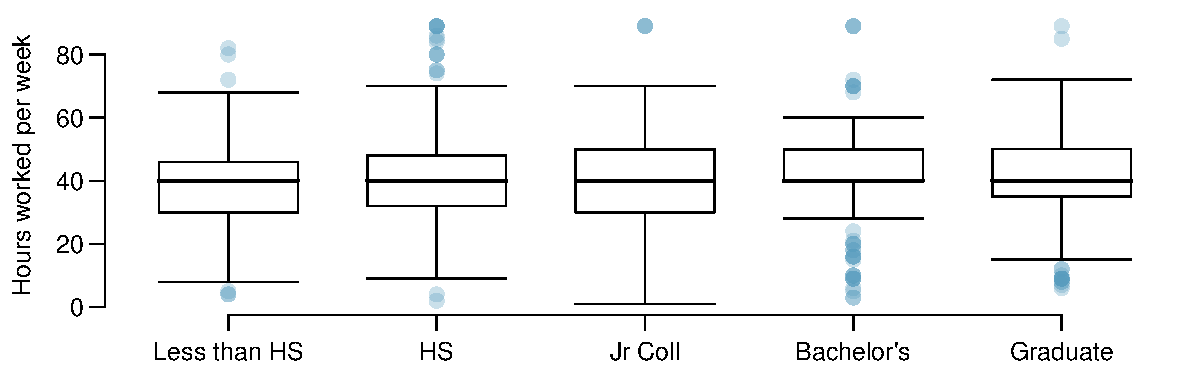
\includegraphics[width=\textwidth]{ch_inference_for_means/figures/eoce/workDeg/workDeg_work_edu_raw_box}
\end{center}
\begin{parts}
\item Write hypotheses for evaluating whether the average number of hours worked varies across the five groups.
\item Check conditions and describe any assumptions you must make to proceed with the test.
\item Below is part of the output associated with this test. Fill in the empty cells.

\begin{center}
\renewcommand{\arraystretch}{1.25}
\begin{tabular}{lrrrrr}
  \hline
 			& Df 	& Sum Sq									& Mean Sq										& F value										& Pr($>$F) \\ 
  \hline
degree	 	& \fbox{\textcolor{white}{{\footnotesize XXXXX}}}	 	& \fbox{\textcolor{white}{{\footnotesize XXXXX}}} 		& 501.54	& \fbox{\textcolor{white}{{\footnotesize XXXXX}}} 	& 0.0682 \\ 
Residuals		& \fbox{\textcolor{white}{{\footnotesize XXXXX}}} & 267,382 	& \fbox{\textcolor{white}{{\footnotesize  XXXXX}}} 			&  		&  \\ 
   \hline
Total			& \fbox{\textcolor{white}{{\footnotesize XXXXX}}} &\fbox{\textcolor{white}{{\footnotesize XXXXX}}}
\end{tabular}
\end{center}

\item What is the conclusion of the test?

\end{parts}
}{}

% 47

\eoce{\qt{True / False: ANOVA, Part I} Determine if the following statements are true or false in ANOVA, and explain your reasoning for statements you identify as false.
\begin{parts}
\item As the number of groups increases, the modified significance level for pairwise tests increases as well.
\item As the total sample size increases, the degrees of freedom for the residuals increases as well.
\item The constant variance condition can be somewhat relaxed when the sample sizes are relatively consistent across groups.
\item The independence assumption can be relaxed when the total sample size is large.
\end{parts}
}{}

\textA{\newpage}

% 48

\eoce{\qt{Child care hours} The China Health and Nutrition Survey aims to examine the effects of the health, nutrition, and family planning policies and programs implemented by national and local governments.\footfullcite{data:china} It, for example, collects information on number of hours Chinese parents spend taking care of their children under age 6. The side-by-side box plots below show the distribution of this variable by educational attainment of the parent. Also provided below is the ANOVA output for comparing average hours across educational attainment categories.
\begin{center}
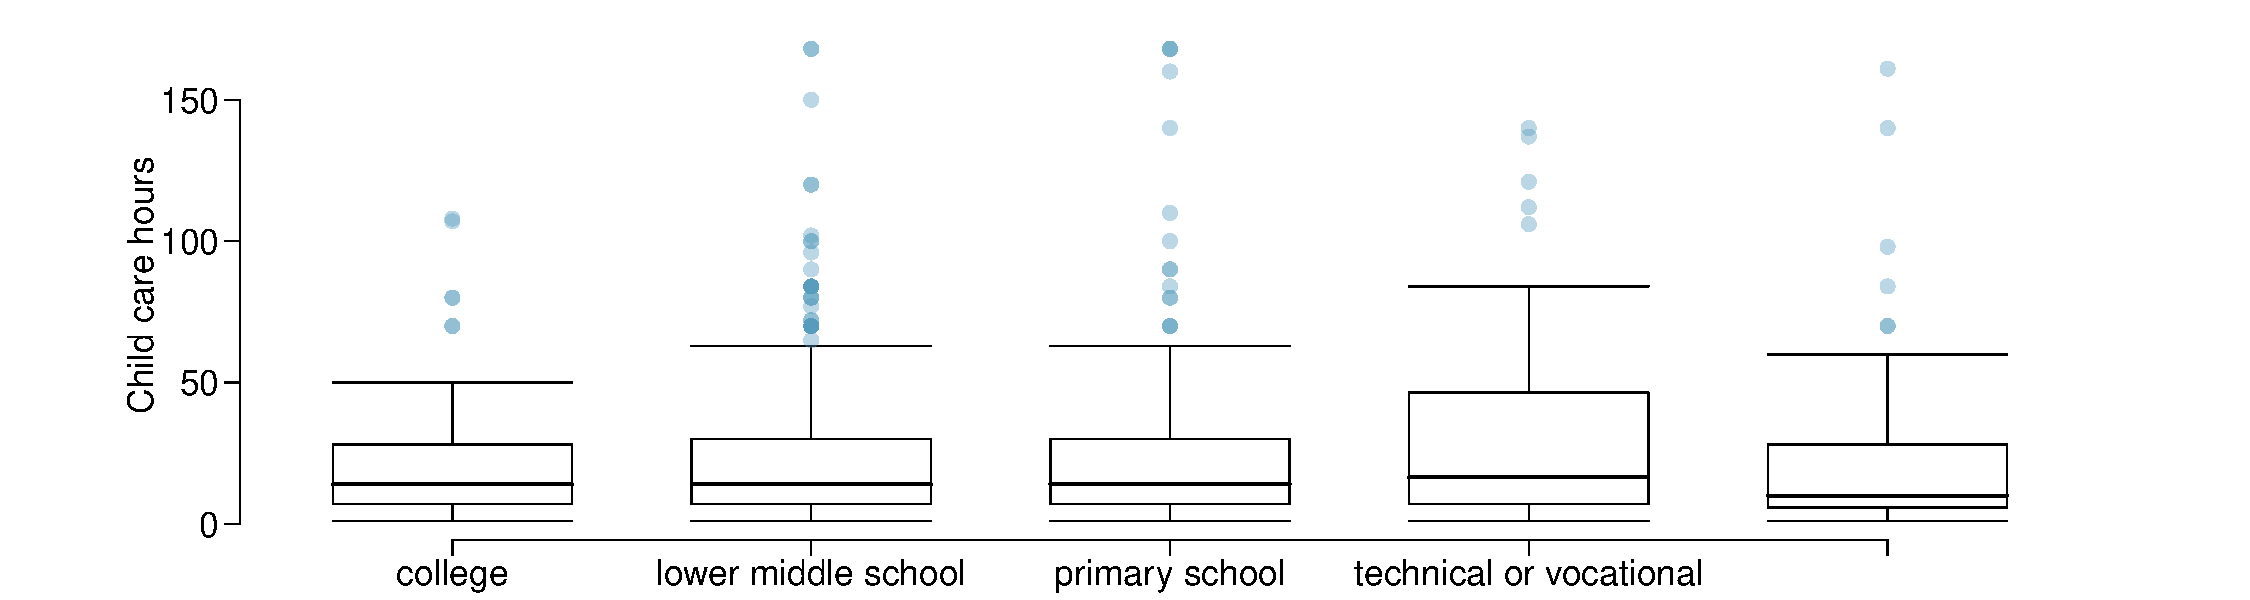
\includegraphics[width=\textwidth]{ch_inference_for_means/figures/eoce/china/china_edu_box}
\end{center}
\begin{center}
\begin{tabular}{lrrrrr}
  \hline
 & Df & Sum Sq & Mean Sq & F value & Pr($>$F) \\ 
  \hline
education & 4 & 4142.09 & 1035.52 & 1.26 & 0.2846 \\ 
  Residuals & 794 & 653047.83 & 822.48 &  &  \\ 
   \hline
\end{tabular}
\end{center}
\begin{parts}
\item Write the hypotheses for testing for a difference between the average number of hours spent on child care across educational attainment levels.
\item What is the conclusion of the hypothesis test?
\end{parts}
}{}

% 49

\eoce{\qt{Prison isolation experiment, Part II} Exercise~\ref{prison} introduced an experiment that was conducted with the goal of identifying a treatment that reduces subjects' psychopathic deviant $T$-scores, where this score measures a person's need for control or his rebellion against control. In Exercise~\ref{prison} you evaluated the success of each treatment individually. An alternative analysis involves comparing the success of treatments. The relevant ANOVA output is given below.
\begin{center}
\begin{tabular}{lrrrrr}
  \hline
 & Df & Sum Sq & Mean Sq & F value & Pr($>$F) \\ 
  \hline
treatment & 2 & 639.48 & 319.74 & 3.33 & 0.0461 \\ 
  Residuals & 39 & 3740.43 & 95.91 &  &  \\ 
   \hline
\multicolumn{6}{r}{$s_{pooled} = 9.793$ on $df=39$}
\end{tabular}
\end{center}
\begin{parts}
\item What are the hypotheses?
\item What is the conclusion of the test? Use a 5\% significance level.
\item If in part~(b) you determined that the test is significant, conduct pairwise tests to determine which groups are different from each other. If you did not reject the null hypothesis in part~(b), recheck your solution.
\end{parts}
}{}

% 50

\eoce{\qt{True / False: ANOVA, Part II} Determine if the following statements are true or false, and explain your reasoning for statements you identify as false.

If the null hypothesis that the means of four groups are all the same is rejected using ANOVA at a 5\% significance level, then ...
\begin{parts}
\item we can then conclude that all the means are different from one another.
\item the standardized variability between groups is higher than the standardized variability within groups.
\item the pairwise analysis will identify at least one pair of means that are significantly different.
\item the appropriate $\alpha$ to be used in pairwise comparisons is 0.05 / 4 = 0.0125 since there are four groups.
\end{parts}
}{}
